\chapter{Moodle általános tudnivalók}

A moodle egy oktatási célokra szolgáló open source web applikáció. A szerveroldali vezérlés PHP nyelven lett implementálva és SQL adatbázist használ. Széles körben elterjedt az ingyenessége és a könnyen bővíthetősége miatt az iskolákban, de még munkahelyeken is használják. Tanulóknak, tanároknak és adminisztrátoroknak is ajánlják, korszerű plug-inek tölthetőek le, személyre szabott oktatási felület hozható létre, a kurzusok dinamikusan változtathatók és így tovább. \par
Ebben a fejezetben a Moodle rendszerről, illetve a Moodle plug-in fejlesztésről lesz leginkább szó.

\section{A Moodle telepítése}

Mivel a Moodle PHP nyelven íródott és SQL szervert használ, így az alábbi dolgokra lesz szükség:
\begin{itemize}
    \item Egy webszerverre, mely támogatja a PHP-t. Ilyen például az Apache vagy a Nginx.
    \item Egy SQL szerverre, mint például a PostgreSQL, MariaDB vagy MySQL.
    \item Ezenkívül a Moodle aktuális forráskódjára, itt viszont érdemes odafigyelni, hogy az utolsó verziószámú Moodle mely PHP és SQL szervereket támogat.
\end{itemize}

A Moodle forráskódját a weblapjukról is be lehet tölteni, de Gitről is le lehet klónozni az alábbi paranccsal:

\begin{center}
git clone --branch MOODLE\_39\_STABLE git://git.moodle.org/moodle.git
\end{center}

Ezután egy böngészőben történő installálást követően már tudjuk is használni.\par
Minden egyes indításkor ellenőrzi a Moodle, hogy az adott pluginek megfelelő verziószámmal rendelkeznek vagy frissíteni kell-e ezeket. Ezután már tudjuk is használni a Moodle kezdőfelületét.

\section{A Moodle felépítése}

A Moodle-ben az M betű a modularitást jelenti. Ez alatt azt értjük, hogy a Moodle egyes részei egyes modulok, ezeket látja a felhasználó. Ezek a modulok kapcsolatban állhatnak egymással, vagy lehetnek teljesen különálló részek. Ezeket a modulokat szokás Plug-innek nevezni. A moodle-ben vannak beépített pluginek, ilyen például a naptár, a quiz, és így tovább. Ezek teszik teszik ki a fájlrendszerének körülbelül a felét, a maradék részt az őket összefogó és irányító rendszerfájlokból adódik. Az alábbi ábra jól illusztrálja ezt:

\begin{center}
    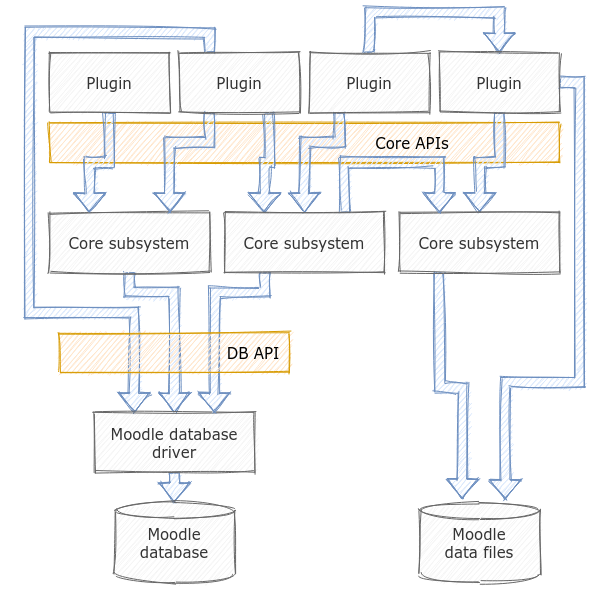
\includegraphics[scale=0.7]{Fejezetek/Images/moodleBuild.png}
\end{center}

\subsection{A pluginek fajtái}

Jelenleg a Moodle-ben 58 fajta plugin létezik, mind teljesen különböző funkcionalitással és szerkezettel. Ezeket a mapparendszerben lévő elhelyezkedésükkel különböztetjük meg egymástól. A plugineken belül lehetnek további típusú pluginek, amelynek a közös tulajdonsága, hogy az alapplugint használja, ezeket a mappán belüli másik mappa fogja meghatározni. Például, ha szeretnénk egy olyan plugint készíteni, amely minden alkalommal a felhasználó kezdőfelületére kiírja egy dobozba, hogy "Hello User", akkor az egy block típusú plugin lesz, és a mapparendszerben a blocks/hellouser mappába kell létrehozni. Néhány plugin köztük fontosabb, többször használtabb, vannak viszont olyanok, amelyek speciálisabbak. Például az Activity modules az egyik legfontosabb, ez maga az oktatási felületet biztosító plugin, így ennek több alpluginja lehet, mint például a Calendar type pluginnak. Néhány fontosabb plugin: 
\begin{itemize}
    \item Activity Module (oktatás, osztályzás), 
    \item Blocks(Alap felület variálása, új állandó tartalom megjelenítése), 
    \item Themes( oktatási felület kinézete, nem csak CSS segítségével), 
    \item Authentication (Regisztráció, bejelentkezés), 
    \item Enrolement (Rangok kiosztása, kurzusok személyeinek beállítása), 
    \item Course (kurzus létrehozása, tananyag feltöltése, tesztek létrehozása), 
    \item Admin (Pluginek kezelése, menedzselése, testreszabása, telepítése és törlése), 
    \item Local (Saját személyes pluginek kezelése, létrehozása) 
\end{itemize}

Természetesen minden plugin, amit a \href{https://moodle.org/plugins/}{Moodle Plugin website}-ról töltünk le, az a Local mappában kerül telepítésre, így a szakdolgozat mappaszerkezete is a local/szakdolgozat formát követi.

\section{Moodle plugin}

\subsection{Közös elemek}

Minden Moodle plugin tartalmaz 3 elemet:
\begin{itemize}
    \item version.php
    \item lang/en/plugintípus\_pluginnév.php
    \item db/install.xml
\end{itemize}

Ezek nélkül a Moodle fel sem telepíti a pluginünket. A version.php felel a pluginek tulajdonságainak meghatározásában, amelyek segítségével ismeri fel a Moodle a különböző modulokat. Két adatot kötelező megadni ebben: a \$plugin->component tartalmazza a plugin azonosítóját, amely mindig a plugintípus\_pluginnév formátum, a másik a \$plugin->version, amely a plugin verziószámát tartalmazza az alábbi formában: YYYYMMDDXX, ahol a YYYY az aktuális évet, az MM az aktuális hónapot, a DD pedig a napot tartalmazza, az XX pedig a jelenleg futó verziószámot, amely mindig 01-gyel kezdődnie. A verziókról később írok részletesen. Egyéb tulajdonságok, amelyeket a version.php-ben határozunk meg:
\begin{itemize}
    \item \$plugin->requires: minimum Moodle verziószám
    \item \$plugin->supported: ajánlott Moodle verziószám
    \item \$plugin->release: mely Moodle verzióra érkezett a plugin
    \item stb.
\end{itemize}

A lang/en/plugintípus\_pluginnév.php tartalmazza azokat a szövegeket, amelyek felhasználunk a plugin elkészítésében. Ezek segítségével nem kell a kódba beleégetni a különböző kiírásokat és feliratokat, hanem ebből a fájl-ból kiolvasva történik meg a behelyettesítés. Ennek a lehetőségnek hála tudunk akár többnyelvű modult létrehozni. Az alapja egy tömb, melyben kulcsként a kulcsszót adjuk meg, értékként megint a megjeleníteni kívánt szöveget. Az index.php-ben pedig a get\_string() metódus segítségével tudjuk kiolvasni. Alapból a Moodle csak az angol nyelvet telepíti fel, így ha szeretnénk magyar nyelvet belerakni, akkor a Site Administration/Administration/Language/Language packs belül kell telepíteni, illetve a lang mappában kell létrehozni egy /hu/plugintípus\_pluginnév.php fájlt és megcserélni az en-ben lévő \$string[] értékeit magyarra. \par

Az utolsó fájl pedig a db/install.xml. Ez a fájl kakukktojás a másik kettőhöz képest, mert ennek a megléte nem szükséges a plugin létrehozásához. Célja, hogy a pluginhez tudjunk táblázatot készíteni, annak pedig az oszlopait és annak értékeit meghatározza. Ezenkívül a fájl tartalmazza még a plugin útvonalát. Amikor telepítjük a plugint, akkor a Moodle adatbázisához hozzáteszi ezt az adatbázist mdl\_plugintípus\_pluginnév néven. Viszont ügyelni kell a plugin törlése esetén az adatbázisban lévő adatok is törlődnek, így biztonsági mentést érdemes végezni, mielőtt eltávolítanánk a saját modulunk.\par

Ezek a legfontosabb közös elemei egy pluginnek, ezenkívül még létezik néhány:
\begin{itemize}
    \item classes/ mappa, amely a pluginben felhasználni kívánt egyedi osztályokat tartalmazza
    \item styles.css, amely az index.php-hoz tartozó css
    \item readme fájl
    \item lib.php, amely az index.php-ban felhasznált függvények tárolására szolgás
    \item stb.
\end{itemize}

\subsection{Dinamikus plugin készítése és főbb elemei}

A Moodle korábban létrejött, mint azok a modern PHP keretrendszerek, amelyek tartalmazzák a a HTTP kérések kezelését és irányítását és létrehozzák a válaszokat is a kérésekkel. Emiatt a Moodle a Page Controller minta segítségével valósítja meg ezt a folyamatot. Ennek működése, hogy minden request egy request handler-en keresztül történik feldolgozásra és innen irányítja tovább a megfelelő könyvtárakba, ahol a feldolgozás és megvalósítás történik, majd a response-t is a request handleren keresztül válaszol a felhasználó számára. A requestek a címsorban történnek tárolásra és ezen keresztül történnek a könyvtárakban az értékadások. Az alábbi illusztráció jól bemutatja a folyamatot:
\begin{center}
    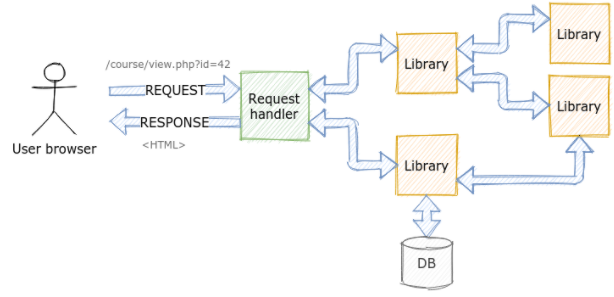
\includegraphics[scale=0.8]{Fejezetek/Images/requestHandler.png}
\end{center}

Ezen keresztül lehet látni, hogy az $id$ adattag megkapja a $42$ értéket, a könyvtárak ezen keresztül lefuttatják a megfelelő függvényeket és a választ a request handleren keresztül közlik a felhasználóval. Hogy el tudjuk érni a request handler-t szükséges elsőnek betölteni a főmappában lévő config.php fájl-t, amely az alábbi parancs segítségével történik: \par
\begin{itemize}
    \item[] require(\_\_DIR\_\_. '/../../config.php');
\end{itemize}

Ez a fájl tartalmazza az adatbázis, session-ök, jelenlegi kurzusok, témák és nyelvek inicializálását és ezekhez kapcsolódó adattagokat, funkciókat. Pontosítva, a config.php-n keresztül történik a többi főbb php file meghívásra, melyeken keresztül tudjuk a Moodle főbb részeit elérni. \par

Ezenkívül biztonsági okokból a fejlesztő nem tudja elérni a \$\_GET,  \$\_POST és  \$\_REQUEST paramétereit, helyette a Moodle biztosít egy require\_param() és optional\_param() függvényeket. Ezek meghívásával tudjuk a megfelelő adattagnak a címsorban lévő értéket felvetetni. A függvényeknek meg kell adni a címsorban szereplő kulcsszót, amely alapján veszik fel az értéket (A példánkban ez az $id$ volt), egy kezdőértéket, ha nem találna ilyet és egy típust, hogy milyen értéket vegyen fel. Ezekből rengeteg típus van, a leggyakoribbak:

\begin{itemize}
    \item PARAM\_INT: Integert váró paraméter
    \item PARAM\_ALPHA: ASCII kódolású, csak betűkből álló rövid stringet vár bemenetnek
    \item PARAM\_ALPHANUM: ASCII kódolású, betűkből és számokból álló rövid stringet vár bemenetnek
    \item PARAM\_BOOL: Egy 0-át vagy 1-et visszaadó érték, mely ha 'off'-t, 'no'-t vagy 'false'-t kap, akkor ad vissza 0-t, ha 'on'-t, 'yes'-t vagy 'true'-t kap, akkor pedig 1-et.
    \item PARAM\_TEXT: UTF-8at támogató nyelv, minden taget lecsupaszítva
    \item PARAM\_PATH: egy úgyvonalat ad vissza.
\end{itemize}

Az összes ilyen típust a lib/moodlelib.php-ben lehet megtalálni és ott vannak a megfelelő tisztító és vezérlőkódok is leprogramozva.

A másik fontos része a pluginünknek, hogy azt a böngésző címsorából közvetlenül ne tudjuk elérni vagy módosítani, hanem csak a könyvtárakon keresztül tudjuk betölteni, ehhez az alábbi sornak kell a kódban lennie: \par
\begin{itemize}
    \item[] defined('MOODLE\_INTERNAL') || die();
\end{itemize}

Ennek segítségével tudjuk megcsinálni, hogy vagy csak a Moodle könyvtár segítségével történjen a betöltés, ha pedig nem sikerült úgy, abban az esetben egy fehér képernyő látszódjon és a console-ból se lehessen kiolvasni semmilyen forráskódot. \par
Minden egyéb betöltést pedig a /classes mappából történik. 

\subsection{Plugin megjelenítése}

Minden Plugin kezdőfelülete az index.php. Ebben hozzuk létre a változóinkat, adunk nekik értéket, jelenítjük meg a plugin tartalmát, és itt állítunk be témát. Minden pluginhez tartozik egy \$PAGE globális változó, amelyen keresztül készítjük el és szabjuk testre a plugint. Egy \$PAGE esetén sok tulajdonságot lehet beállítani, viszont első körben nézzük meg a legfontosabbakat. \par
Elsőnek állítsuk be a \$PAGE URL címét: 
\begin{itemize}
    \item[] \$PAGE->set\_url(new moodle\_url('/plugintípus/pluginnév/index.php));
\end{itemize}

Ezzel a függvényhívással már tudunk hivatkozni a jelenlegi címre, illetve a plugin indításakor a Moodle tudni fogja, hogy melyik címet kell megnyitnia. Később is hasznos lehet nekünk ez, mivel például ha szeretnénk egy form-ot létrehozni, akkor a fejléc lehet az alábbi:
\begin{itemize}
    \item[] echo '<form method="get" action="'.\$PAGE->url.'">';
\end{itemize}

A másik nagyon fontos, hogy megadjuk, hogy a \$PAGE mihez tartozik, a Moodle mely részével van összekötve, összekapcsolva. Itt értem ez alatt, hogy plugin egy modulhoz, egy kurzushoz vagy magához a rendszerhez van készítve, azon részeivel van kapcsolatban. Ezt a következő módon tudjuk megvalósítani:

\begin{itemize}
    \item[] \$PAGE->set\_context(context\_system::instance());
\end{itemize}

Ebben az esetben egy rendszerszintű plugint fogunk érteni. Ha kurzushoz akarjuk, akkor paraméternek a contect\_course::instance(\$kurzusid)-t, ha pedig egy modulhoz, akkor a contect\_module::instance(\$moduleid)-t kell megadni. \par

Ezeket kötelező beállítani minden \$PAGE esetén, de vannak még olyan tulajdonságok, amelyek fontosak. A
\begin{itemize}
    \item[] \$PAGE->set\_title(get\_string('pluginname', 'plugintípus\_pluginnév'));
\end{itemize}

segítségével a böngésző tetején a füleknek a nevét lehet beállítani, itt is a \break lang/en/plugintípus\_pluginnév-ből veszi ki a pluginname kulcsú értéket és azt állítja be, a 
\begin{itemize}
    \item[] \$PAGE->set\_heading(get\_string('heading', 'plugintípus\_pluginnév'));
\end{itemize}
segítségével tudunk címet adni a pluginnak, ez is ugyannazzal a módszerrel történik, mint a title esetén, végül pedig a
\begin{itemize}
    \item[] \$PAGE->set\_pagelayout('standard');
\end{itemize}
függvényhívás segítségével tudjuk kiválasztani, hogy mely beépített alapkinézetet szeretnénk választani. Nagy többségében a 'standard' kinézetet választják, de ebből is többféle létezik: 'base','course','admin','login',stb. \par

Ha pedig mindent sikerült beállítani, akkor ezeket már csak ki kell írni a képernyőre. Ebben segít a \$OUTPUT változó, amely a renderelésért felel, ezen változó függvényeinek meghívásával történnek meg a kiíratások, megjelenítések. Például eddig bemutatott \$PAGE adattagok értékeit beállítottuk, ennek megjelenítésére a 
\begin{itemize}
    \item[] echo \$OUTPUT->header();
\end{itemize}
meghívásával tudjuk megjeleníteni. A lábléc-et az
\begin{itemize}
    \item[] echo \$OUTPUT->footer();
\end{itemize}
parancs szükséges, viszont a index.php "törzséhez" nem kell külön az \$OUTPUT változó egy függvényét meghívni, elég ha megfelelő echo és html tagek közt megadjuk. Viszont célszerű speciális esetekben a Moodle által létrehozott kiírató függvényeket használni. Ezeket az eseteket a következő ábra bemutatja:

\begin{center}
    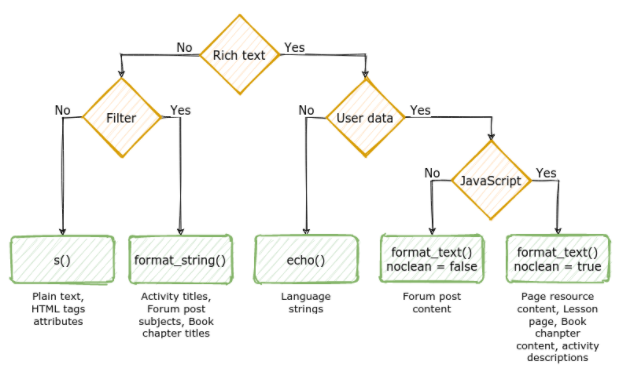
\includegraphics[scale=0.9]{Fejezetek/Images/print.png}
\end{center}

Ezenkívül lehetőségünk van különböző HTML megjelenítést és logikai elkülönítést segítő függvényeket is meghívni, ezt a html\_writer osztály-ban lévő függvények segítségével tudjuk megtenni. Például
\begin{itemize}
    \item[] echo html\_writer::tag('input','nev',[ 'type' => 'text', 'name' => 'username']); 
\end{itemize}
kiíratás segítségével egy új input taget tudubk létrehozni, amely szöveget vár, username néven tárolja el és a kezdőértéke a nev szöveg. Ilyen függvényekből is több fajta létezik: link(), img(), table(), stb.

\subsection{Egyéb beállítások}

A Moodle-ben van lehetőségünk még rengeteg dologra egy plugin készítésével kapcsolatban. Lehet
\begin{itemize}
    \item Fő menüsorra elhelyezni, vagy almenüsorra beszúrni,
    \item Admin felhasználói beállításokat lehet adni, amelyek segítségével testreszabható a plugin,
    \item Verziókövetés, 
    \item Adatbázist lehet hozzákapcsolni és abból SQL lekérdezések segítségével lehet az adatokat kinyerni,
    \item stb.
\end{itemize}

Ezekkel azért nem foglalkozunk komolyabban, mivel a szakdolgozat nem dolgozza fel, így csak említés és rövid áttekintésként vesszük végig. \par

A menübár egy fa struktúrával felépített UI amelynek 3 részét különböztetjük meg:
\begin{itemize}
    \item Navigálásért szolgáló bár, amely a kurzusok, órák és ahhoz tartozó oldalak között lehet lépegetni.
    \item Jelenlegi bár, amely az aktuális bárt jeleníti és tárolja
    \item Beállítás bár, amely egy kurzushoz, órához, stb.-hez tartozó beállítások és funkciók megjelenítésével foglalkoznak.
\end{itemize}

Ha szeretnénk az oldalhoz menüsort beállítani, azt a \$PAGE->navigation->add() függvény meghívásával tudjuk megtenni, amelybe egy linket kell belemásolni, illetve ha szeretnénk saját menübárt, akkor azt a lib.php fájlban kell függvények formájában implementálni. Ha pedig szeretnénk a főoldalon található navigation bar-ba elhelyezni, akkor az alábbi kódot kell a lib.php-ban elhelyezni: 

\begin{lstlisting}[language=PHP]
/**
 * Add link to index.php into navigation drawer.
 *      
 * @param global_navigation $root Node representing the global navigation tree.
 */
function plugintipus_pluginnev_extend_navigation(global_navigation $root) {

    $node = navigation_node::create(
        get_string('sayhello', 'plugintipus_pluginnev'), 
        new moodle_url('/plugintipus/pluginnev/index.php'),
        navigation_node::TYPE_CUSTOM,
        null,
        null,
        new pix_icon('t/message', '')
    );
    $node->showinflatnavigation = true;

    $root->add_node($node);
}
\end{lstlisting}

Az adminisztrátori beállításokat a settings.php-ban kell létrehozni, a fejlesztői beállításokat a config.php-ban. Ezek alapján könnyebben szét lehet szedni, hogy melyek a plugin tényleges működése és melyek annak tesztelésére szolgálnak. A configban történt módosításokat és adattagok értékeinek tárolására a config tábla van fenttartva és a \$CFG adattagban történik a meghívása. Ebben tudjuk a get\_config() és set\_config() segítségével lekérni és módosítani. Az adminisztrációs beállítások az admin\_category fa struktúrájú objektumban tárolódnak, melynek a gyökéreleme az \$ADMIN objektum és ezen keresztül tudjuk lekérni változókat. \par

A verziókövetés a version.php file-ban történik. Miven verziószám az alábbi alakban nézz ki YYYYMMDDXX. Ha történik valamilyen szignifikáns változtatás, például adatbázisséma változás, egy új adatbázis létrehozása vagy új elem hozzáadása, akkor léptetni kell a verziószámot egyaránt. A Moodle-ben nincs arra lehetőség, hogy a verziószámot csökkentsük, mindig a következő verziónak "nagyobbnak" kell lennie, mint az aktuális. A nagyobb alatt azt értjük, hogy vagy a dátumnak kell frissebbnek lennie, mint az előző verziószámban lévő, vagy ha a dátum megegyezik, akkor az XX helyén lévő számnak kell nagyobbnak lennie az előzőnél. Ezenkívül az XX helyén lévő számok segítségével tudunk új irányutakat létrehozni a plugin fejlesztésében. \par

Végezetül pedig adatbázisokat lehet egy pluginhez hozzákapcsolni, azon keresztül szerkeszteni és lekérdezéseket indítani. A Moodle-ben egy adatbázis létrehozásához és módosításához létrehozott egy XMLDB editort, hogy azon keresztül generáljon XML fájlokat és azok megfeleljenek a Moodle-ben használt szabályoknak. Ezt a Portálkezelés -> Fejlesztés -> XMLDB-szerkesztő-n keresztül tudjuk elérni. Ezekhez tartozó szabályokból sok van, néhány közülük:

\begin{itemize}
    \item Minden táblának a neve az alábbi módon kell kinéznie: plugintípus\_pluginnév\_tárolniKívántAdat.
    \item Minden táblának kell lennie egy automatikusan léptetett számlálóval.
    \item Minden tábla nevének hossza maximum 28 karakter.
    \item Minden oszlop nevének hossza maximum 30 karakter.
    \item Minden tábla- és oszlopnévnek kerülnie kell a Moodle-ben létrehozott kulcsszavakat.
    \item stb.
\end{itemize}

Minden adatbázis a \$DB változóban. Ehhez include-olni kell a gyökérkönyvtárban található config.php file-t. Ezen a változón keresztül lehet indítani táblázatmódosításokat és lekéréseket. Rengeteg előre gyártott függvénnyel rendelkezik, mint például a get\_records\_sql(), count\_records(), record\_exists és így tovább. 